\documentclass{beamer}
% \usetheme{Boadilla}
\usetheme{Copenhagen}

\usepackage[utf8]{inputenc}

\usepackage[bibstyle=ieee,citestyle=numeric-comp]{biblatex}
\usepackage[title, titletoc]{appendix} %improved appendix controls

\usepackage{amsmath} %MATHS
\usepackage{amssymb}

\usepackage{float} %float placement
\usepackage[font={small}, justification=centering]{caption}
\usepackage{subcaption} % subfigure package
\usepackage[export]{adjustbox}
\usepackage{pdfpages} %integrate other pdf's 
\usepackage{graphicx} %image insertion
% \usepackage{minted} %auto code formatting for multiple languages
\usepackage[newfloat]{minted} %auto code formatting for multiple languages
% \usepackage{enumitem}
\usepackage{multirow} % for table formatting

\usepackage{color,soul} % used for highlighting
\usepackage{xcolor}	%more colors
% \usepackage{sectsty}

% \usepackage{titlesec} # breaks for presentation
% \usepackage{todonotes} %reminders
\usepackage{blindtext} % text for document formatting
\usepackage{comment} %block comments
% \usepackage[firstpage=true]{background}

% \usepackage[hidelinks, breaklinks]{hyperref} %improved referencing; already included for presentations
\usepackage[capitalise, nameinlink, noabbrev, english]{cleveref}

%extra set-up
% !TeX spellcheck = en_GB
\graphicspath{{images/}}
\addbibresource{bibliography.bib}

% environments and functions
% \newenvironment{code}{\captionsetup{type=listing}}{} % code environment that can page-break
% \SetupFloatingEnvironment{listing}{name=Source Code}
% \definecolor{bg}{rgb}{0.95,0.95,0.95}


\title{LaTeX Tutorial}
\author{Jacob White}
\institute{Memorial University of Newfoundland}
\date{May 7, 2021}

\begin{document}

\begin{frame}
    \titlepage
\end{frame}

% \begin{frame}{Table of Contents}
%     \tableofcontents
% \end{frame}

\section{Starting Notes}

\begin{frame}{Scope}

    \begin{itemize}
        \item This will be more of a starter to give you the gist of how to get going
        \item Lots of nuance - not feasible to teach all of the ins and outs of \LaTeX
    \end{itemize}
    
\end{frame}

\subsection{Useful Resources}
\begin{frame}{Editors}

    \textbf{RECOMMENDATION}\\
    \begin{itemize}
        \item Overleaf (online): \url{https://www.overleaf.com}
    \end{itemize}
    \vspace{\baselineskip}
    
    \textbf{Others} (\textit{substantially} more inconvenient to set up!)\\
    \begin{itemize}
        \item MiKTeX: \url{https://miktex.org/}
        \item Visual Studio Code w/ LaTeX Workshop extension
    \end{itemize}
    
\end{frame}

\begin{frame}{Revision and Comments}

    \textbf{GitHub}
    \begin{itemize}
        \item A repository can be used for tracking changes between people (us and Sarah) 
        \item Built in functionality with Overleaf
    \end{itemize}
    
    \vspace{\baselineskip}
    
    \textbf{Grammarly}
    \begin{itemize}
        \item Can help you proof/revise your writing quickly
        \item \url{https://www.engr.mun.ca/techcomm/wp-content/uploads/2020/09/GrammarlyPremiumInstructions.pdf}
    \end{itemize}
    
\end{frame}

\begin{frame}{Examples}

    \begin{itemize}
        \item Easiest way to get started making \LaTeX documents is to bootstrap yours from examples
        \item I'll send out an email with some of my previous work that you can pick through
    \end{itemize}
    
\end{frame}

\subsection{Golden Rule}

\begin{frame}{When your unsure how to do something in \LaTeX... }
    
    \begin{itemize}
        \item Google your question, followed by `latex'
        \item This works 95\% of the time, Latex is old so there are lots of answers out there!
        \item The Tex stack exchange is a great source too: \url{https://tex.stackexchange.com/}
    \end{itemize}
    
\end{frame}


\section{The Basics}
\subsection{Syntax}

\begin{frame}{The \LaTeX `Language'}
    
    \begin{itemize}
        \item You'll notice many similarities to coding languages
        \item Using latex, you structure how the document looks using \textit{commands} and \textit{environments}
        \item Additional features can be added using \textit{packages}
        \item We'll learn how to use all of these by making an document throughout this presentation
    \end{itemize}
    
\end{frame}

\begin{frame}[fragile]{Commands}

    The syntax for using commands is as follows:

    \begin{minted}{tex}
\commandname[optional arguments]{required arguments}
    \end{minted}
    \vspace{\baselineskip}
    
    Some examples:
    \begin{minted}{tex}
\tableofcontents
\pagenumbering{arabic}
\usepackage[bibstyle=ieee]{biblatex}
    \end{minted}
    
\end{frame}

\begin{frame}[fragile]{Environments}

    Used to encapsulate specific formatting and regions of the document, such as figures, tables, math, etc.
    \vspace{\baselineskip}
    
    \begin{minted}{tex}
\begin{document}
    ...
\end{document}
    \end{minted}
    \vspace{\baselineskip}
        
    You can also used a stared (*) version if you don't want it to be numbered
    \vspace{\baselineskip}
    
    \begin{minted}{tex}
\begin{equation*}
    ...
\end{equation*}
    \end{minted}
    
\end{frame}

\subsection{Preamble Essentials}
\begin{frame}[fragile]{Document Classes}
    
    \begin{itemize}
        \item The first thing in any document
        \item Many types:
        \begin{itemize}
            \item article (most common)
            \item pdfathesis (for writing thesis)
            \item beamer (for presentations, i.e. this!)
            \item etc.
        \end{itemize}
    \end{itemize}
    \vspace{\baselineskip}
    
    \begin{minted}{tex}
  \documentclass{beamer}
  \documentclass[12pt]{article}
    \end{minted}
    
\end{frame}

\begin{frame}[fragile]{Packages}
    As mentioned, packages are how you can add additional functionality to \LaTeX\\
    
    For example, here is how you can alter the proportions of you paper:
    \vspace{\baselineskip}
    
    \begin{minted}{tex}
\usepackage[paper=letterpaper, margin=1in]{geometry}
    \end{minted}
    
\end{frame}


\section{Writing your document}
\begin{frame}[fragile]{Beginning your Doc}

    So far, everything shown has been preamble - things will only show up once you put in:
    \vspace{\baselineskip}

    \begin{minted}{tex}
\begin{document}
    ...
\end{document}
    \end{minted}
    \vspace{\baselineskip}
    
    The entire written document must be within this environment
    
\end{frame}

\subsection{Basic Writing}
\begin{frame}[fragile]{Sectioning}
    To divide up your document, we use \textit{sections}. You can further subdivide using \textit{subsections}, and \textit{subsubsections}.
    \vspace{\baselineskip}
    
    \begin{minted}{tex}
- \section{Section Name}
- \subsection{This is a subsection}
- \subsubsection{This is a subsubsection}
    \end{minted}
    \vspace{\baselineskip}
    
    \begin{figure}[H]
        \centering
        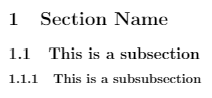
\includegraphics{images/sections.png}
    \end{figure}
    
\end{frame}

\begin{frame}[fragile]{Writing}
    
    There's nothing too complicated when it comes to writing actual words down in latex, you just have to have them placed in the correct \textbackslash{}section\{\} of the document.\\
    
    There are some restricted characters that can't be typed on their own such as \_ \% \& \textbackslash{} \{ \} \$, and need to be typed like so,\\
    
    \begin{minted}{tex}
\_ \% \& \textbackslash \{ \} \$
    \end{minted}
    
\end{frame}

\begin{frame}{Writing}

    To end a line use a double-backslash, \textbackslash\textbackslash \\ 
    
    To end a paragraph, use \textbackslash{}par \\
    
    To add a space between lines or paragraphs, you have to and a black new-line after the \textbackslash\textbackslash
    
\end{frame}

\begin{frame}[fragile]{Referencing Objects}

    Oftentimes, you'll want to refer to figures or tables within your document. This is easily done in latex as it automatically orders and numbers these objects for you.\\
    
    There are a few packages that improve the default object referencing that I recommend:
    \vspace{\baselineskip}
    
    \begin{minted}[fontsize=\footnotesize, breaklines]{tex}
\usepackage[hidelinks, breaklinks]{hyperref}
\usepackage[capitalise, nameinlink, noabbrev, english]{cleveref}
    \end{minted}
    
\end{frame}

\begin{frame}[fragile]{Referencing Objects}

    \begin{itemize}
        \item To make a referencing point, use the \textbackslash{}label\{labelName\} command (many examples coming up)
        \item To refer back to this point, use \textbackslash{}cref\{labelName\}. 
        \begin{itemize}
            \item Say you are referencing a figure, the result will be: `Figure 7'
        \end{itemize}
        \item If you don't want the `Figure' part to appear, use the \textbackslash{}ref\{\} command instead
    \end{itemize}
    
    
    
    
    
\end{frame}

\subsection{Figures}
\begin{frame}[fragile]{Figures Packages}

    The following packages are required:
    \vspace{\baselineskip}

    \begin{minted}[breaklines]{tex}
\usepackage{graphicx} %for images
\usepackage[font={small}, justification=centering]{caption} % caption style
\usepackage{float} %float placement
\usepackage{subcaption} % for subfigures 
    \end{minted}
    
\end{frame}

\begin{frame}{Figures}

    As seen in \cref{fig:eg_figure_label}, you can add in images using figures.

    \begin{figure}[H]
        \centering
        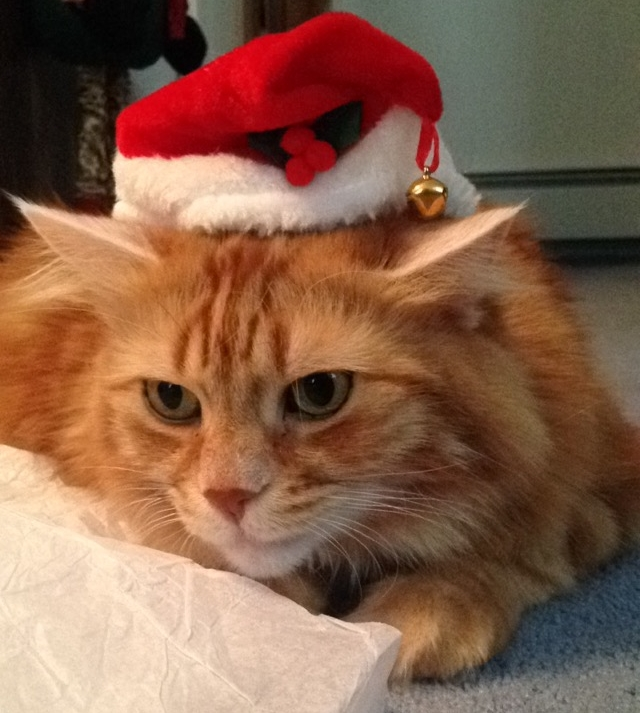
\includegraphics[scale=0.1]{images/example_image.JPG}
        \caption{The caption goes in here.}
        \label{fig:eg_figure_label}
    \end{figure}
    
\end{frame}

\begin{frame}[fragile]{Figure structure}
    
    To make the figure in the previous slide, the below was used:
    \vspace{\baselineskip}
    
    \begin{minted}[fontsize=\small]{tex}
\begin{figure}[htbH]
    \centering
    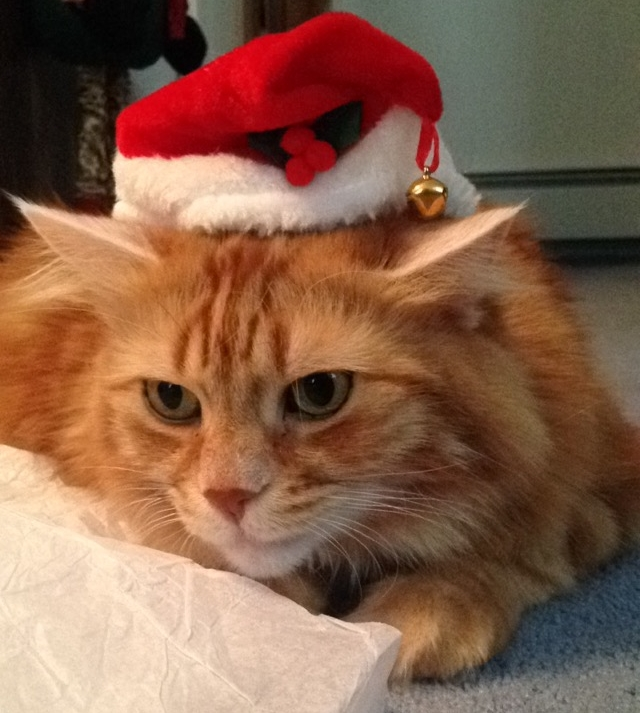
\includegraphics[scale=0.1]{images/example_image.JPG}
    \caption{The caption goes in here.}
    \label{fig:eg_figure_label}
\end{figure}
    \end{minted}
    
\end{frame}

\begin{frame}{Sub-Figures}
    
    You can also have multiple images per figure if they are related, such as \cref{fig:eg_sub_figure}.

    \begin{figure}[H]
        \centering
        \begin{subfigure}[c]{0.29\textwidth}
            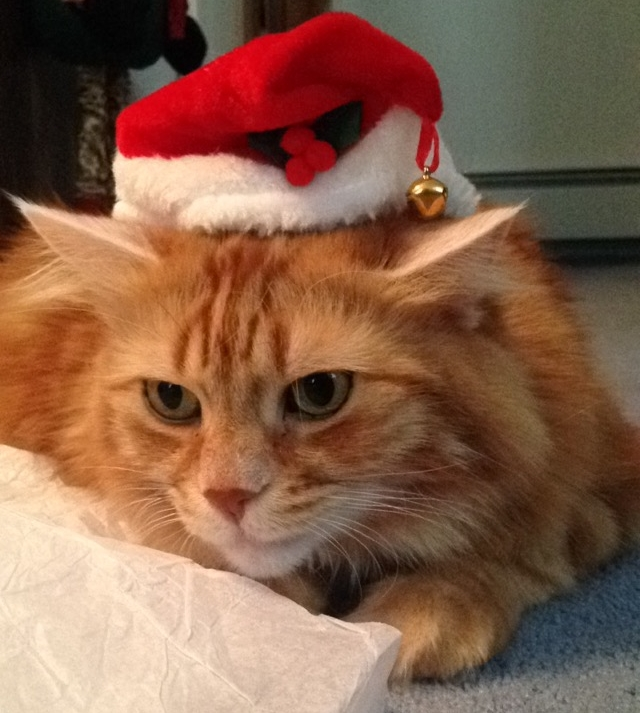
\includegraphics[width=\textwidth]{images/example_image.JPG}
            \caption{}
        \end{subfigure}
        \begin{subfigure}[c]{0.3\textwidth}
            
\includegraphics[width=\textwidth]{images/example_image_2.jpg}
            \caption{}
        \end{subfigure}
        \caption{(a) A cat in a hat. (b) A cat in a box.}
        \label{fig:eg_sub_figure}
    \end{figure}
    
\end{frame}

\begin{frame}[fragile]{Sub-Figures structure}
    
    \begin{minted}[breaklines, fontsize=\small]{tex}
\begin{figure}[H]
    \centering
    \begin{subfigure}[c]{0.29\textwidth}
        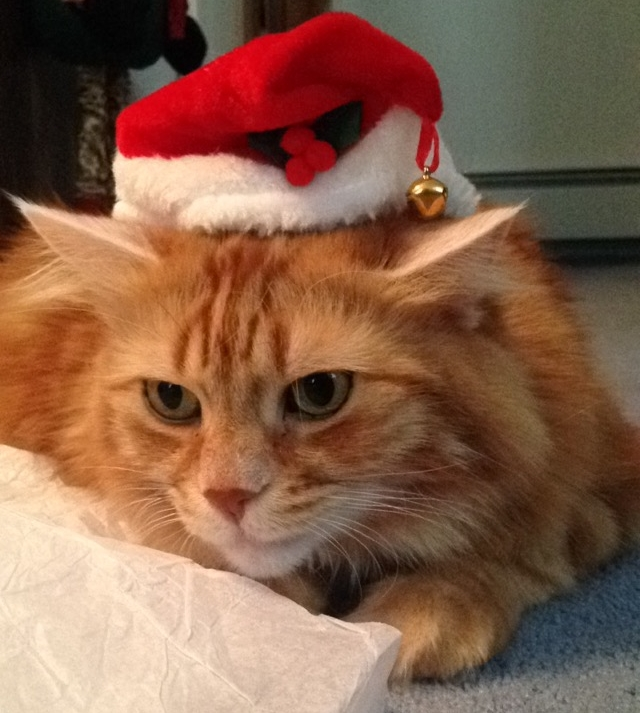
\includegraphics[width=\textwidth]{ images/example_image.JPG}
        \caption{}
    \end{subfigure}
    \begin{subfigure}[c]{0.3\textwidth}
        
\includegraphics[width=\textwidth]{ images/example_image_2.jpg}
        \caption{}
    \end{subfigure}
    \caption{(a) A cat in a hat. (b) A cat in a box.}
    \label{fig:eg_sub_figure}
\end{figure}
    \end{minted}
    
\end{frame}

\subsection{Tables}
\begin{frame}{Tables}
    
    Latex can format your tables, like the example seen in \cref{tab:table_eg}
    
    \begin{table}[H]
        \centering
        \begin{tabular}{c|c|c}
            Filter Order & PFE Error [dB] & LS Error [dB] \\ \hline
            (50/50) & 1.97972e-10 & 1.95831e-10 \\ \hline
            (100/100) & 0.00761004 & 7.18605e-09 \\ \hline
            (150/150) & 4.17774 & 8.00024e-05 \\ \hline
            (200/200) & 4.85818 & 9.27059e-09 \\ \hline
            (1000/1000) & 4.44133 & 1.00683e-07 \\ \hline
        \end{tabular}
        \caption{The mean absolute dB error for the \textbf{room response} for various filter orders.}
        \label{tab:table_eg}
    \end{table}
    
\end{frame}

\begin{frame}[fragile]{Table Structure}

    \begin{minted}[breaklines, fontsize=\small]{tex}
\begin{table}[H]
    \centering
    \begin{tabular}{c|c|c}
        Order & PFE Error [dB] & LS Error [dB] \\ \hline
        (50/50) & 1.97972e-10 & 1.95831e-10 \\ \hline
        (100/100) & 0.00761004 & 7.18605e-09 \\ \hline
        (150/150) & 4.17774 & 8.00024e-05 \\ \hline
        (200/200) & 4.85818 & 9.27059e-09 \\ \hline
        (1000/1000) & 4.44133 & 1.00683e-07 \\ \hline
    \end{tabular}
    \caption{The mean absolute dB error for the \textbf{room response} for various filter orders.}
    \label{tab:table_eg}
\end{table}
    \end{minted}
    
\end{frame}

\subsection{Math}
\begin{frame}[fragile]{Math Packages}
    Two incredibly useful packages for math formatting in LaTeX:
    \vspace{\baselineskip}
    
    \begin{minted}{tex}
\usepackage{amsmath}
\usepackage{amssymb}
    \end{minted}
    
\end{frame}

\begin{frame}[fragile]{Ways to write math}
    Math can be written inline and in block environments: \\
    
    For \textbf{inline}, surround the math in \$: \\
    
    \begin{minted}[fontsize=\small]{tex}
Radial frequency is, $\Omega = 2\pi f$
For proper sampling, $f_{s} > 2\cdot f_{m}$
    \end{minted}
    \vspace{\baselineskip}
    
    Radial frequency is, $\Omega = 2\pi f$ \\
    For proper sampling, $f_{s} > 2\cdot f_{m}$ \\
    
\end{frame}

\begin{frame}[fragile]{The Math Environment}
    
    For standalone equations use the \textit{equation} environment, like in \cref{eqn:eg_equation}:
    
    \begin{equation}
        H(z^{-1}) = \sum_{l=1}^{L} \frac{ b_{0,l} + b_{1,l}z^{-1} }{ 1 + a_{1,l}z^{-1} + a_{2,l}z^{-2} } + \sum_{k=0}^{K}f_{k}z^{-k}
        \label{eqn:eg_equation}
    \end{equation}
    
    \begin{minted}[breaklines, fontsize=\small]{tex}
\begin{equation}
    H(z^{-1}) = \sum_{l=1}^{L} \frac{b_{0,l} + b_{1,l}z^{-1}}{1 + a_{1,l}z^{-1} + a_{2,l}z^{-2}} + \sum_{k=0}^{K}f_{k}z^{-k}
    \label{eqn:no_del_par}
\end{equation}
    \end{minted}
    
\end{frame}

\begin{frame}[fragile]{Multi-Line Equations}

    Equations can be broken into multiple lines, like in \cref{eqn:eg_split}:
    
    \begin{equation}
        \begin{split}
            y + 2x & = 7x + 5 \\
            y & = 5x + 5 \\
            y & = 5(x+1)
        \end{split}
        \label{eqn:eg_split}
    \end{equation}
    
    \begin{minted}[fontsize=\small, baselinestretch=1]{tex}
\begin{equation}
    \begin{split}
        y + 2x & = 7x + 5 \\
        y & = 5x + 5 \\
        y & = 5(x+1)
    \end{split}
    \label{eqn:eg_split}
\end{equation}
    \end{minted}
    
\end{frame}

\begin{frame}{Notes about math usages}
    
    \begin{itemize}
        \item The math environments are what you can use for subscripts and superscripts in text, eg. May $7^{th}, 2021$
        \item You can only use the Greek characters within math environments, eg. $\alpha, \beta, ..., \omega$
    \end{itemize}
    
\end{frame}

\subsection{Other Environments}
\begin{frame}{Lists}

    \begin{itemize}
        \item For unnumbered lists (like this), use the \textit{listing} environment
        \item (Unnumbered list item)
    \end{itemize}
    
    \vspace{\baselineskip}

    \begin{enumerate}
        \item For numbered lists (like \textit{this}), use the \textit{enumerate} environment
        \item (Numbered list item)
    \end{enumerate}

\end{frame}

\section{Citations and Bibliography Management}
\begin{frame}{Using Bibtex for Bibliography Management}
    Possibly the best reason to start using Latex! Bibtex streamlines citations and bibliography's in your work.
\end{frame}

\section{Final Notes}

\end{document}
